\documentclass[11pt]{beamer}
\usetheme{Berlin}
\usepackage[utf8]{inputenc}
\usepackage[francais]{babel}
\usepackage[T1]{fontenc}
\usepackage{amsmath}
\usepackage{amsfonts}
\usepackage{amssymb}
\usepackage{graphicx}
\author{François MALENFER, Danaël CARBONNEAU}
\title{Devoir de programmation}
%\setbeamercovered{transparent} 
%\setbeamertemplate{navigation symbols}{} 
%\logo{} 
%\institute{} 
%\date{} 
\usepackage{xcolor}
\usepackage{listings}
\usepackage{algorithm,algorithmic}

\definecolor{darkWhite}{rgb}{0.94,0.94,0.94}


	
 
\lstset{
  aboveskip=3mm,
  belowskip=-2mm,
  backgroundcolor=\color{darkWhite},
  basicstyle=\footnotesize,
  breakatwhitespace=false,
  breaklines=true,
  captionpos=b,
  commentstyle=\itshape \color{teal},
  extendedchars=true,
  framexleftmargin=16pt,
  framextopmargin=3pt,
  framexbottommargin=6pt,
  frame=tb,
  keepspaces=true,
  keywordstyle=\bfseries \color{orange},
  otherkeywords={module,open,Int32,val},
  language=caml,
  morekeywords={*,...},
  numbers=left,
  numbersep=10pt,
  numberstyle=\tiny\color{teal},
  rulecolor=\color{black},
  showspaces=false,
  showstringspaces=false,
  showtabs=false,
  stepnumber=1,
  stringstyle=\color{gray},
  tabsize=4,
  title=\lstname,
}	

\usepackage{multicol}


 \mode<presentation> {
     \beamertemplatenavigationsymbolsempty
     \setbeamertemplate{footline}[frame number]
   }
\begin{document}

\begin{frame}


\center 
\bigskip


{ \huge \bfseries \color{teal} Devoir de Programmation }
\textbf{Algorithmique Avancée}

{\color{darkgray} François Malenfer (28706664), Danaël Carbonneau (28709878)}

\medskip

\begin{large}

{\fontfamily{lmtt}\selectfont
Implémentation de structures de données de recherche (en OCaml)\cite{leroy3ocaml}
}
\end{large}

\end{frame}


 \section{Introduction}


\begin{frame}[fragile]{Représenter des entiers 128 bits en OCaml}


\begin{lstlisting}
open Int32;;
type entier128 = 
(Int32.t * Int32.t * Int32.t * Int32.t);;
\end{lstlisting} 

\begin{lstlisting}
val cmp : t -> t ->int

val inf : t -> t -> bool

val eg : t -> t -> bool
\end{lstlisting} 


\end{frame}

\section{Tas Minimum}

\begin{frame}[fragile]{Structures\cite{DataStructure}}


\bigskip \begin{lstlisting}
(*indice dernier element * taille du tableau * tableau*)
type heapArray = int ref * int ref * (Int128.t option) Array.t;;

(* N of  rang * ndescendants * elt * fg * fd *)
type  heapTree = E | L of Int128.t | N of int * int *  Int128.t *  heapTree *  heapTree;;
\end{lstlisting} \bigskip


\end{frame}

\begin{frame}[fragile]{Construction\cite{ACM}}
%algo + complexité
\begin{columns}[t]
  \begin{column}{5cm}
  
    \includegraphics[width=6cm]{../Images/graphes/tas_tab_cons_non_ordonné.png} 
    
    \begin{center}
    \medskip
    \;\;\;\;\;\;\;\;\; $\Downarrow$
    \medskip
    \end{center}
    

  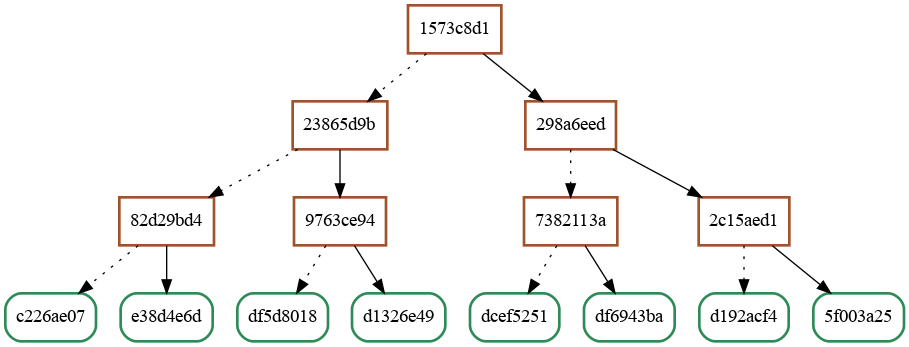
\includegraphics[width=6cm]{../Images/graphes/tas_arbre_cons.png} 



  \end{column}
  
  \begin{column}{5cm}
  
  \begin{scriptsize}
  
    \begin{align}
C &= \sum_{i = 0}^{h-1} 2^i (h - 1 - i)\\
&=  \sum_{j = 0}^{h-1} 2^{h-1-j} j\\
&= 2^{h-1} \sum_{j=0}^{h-1} 2^{-j} j\\
&= 2^{h-1} \sum_{j=0}^{h-1} j \frac{1}{2^j} \\
&= O(2^{h-1})\\
&= O(n)
\end{align}
  \end{scriptsize}


  
  
  \end{column}
 \end{columns}  
\end{frame}

\subsection{Complexités}
\begin{frame}{Ajouts Itératifs}
Formule pour la régression : $(ax +b) (log (mx +c))$

\begin{columns}[t]
  \begin{column}{5cm}
  
\begin{figure}[hbtp]
\centering
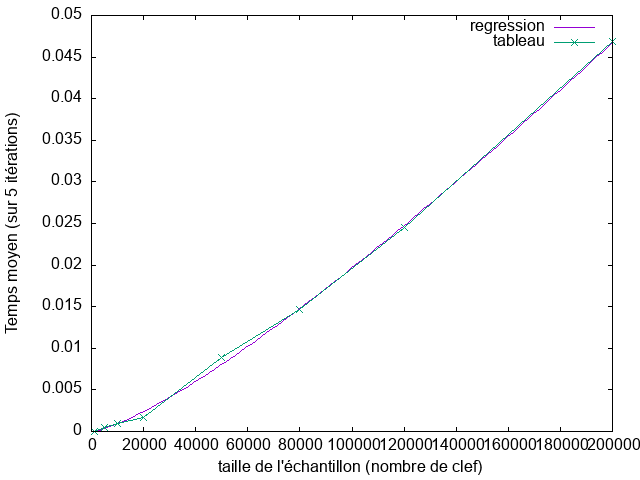
\includegraphics[width=5cm]{../Images/svg courbes pour rapport/regression_ajout_iteratif_tab.png}
\caption{Tas sous forme de tableau}
\label{fig1}
\end{figure}


  \end{column}
  
  \begin{column}{5cm}
  
\begin{figure}[hbtp]
\centering
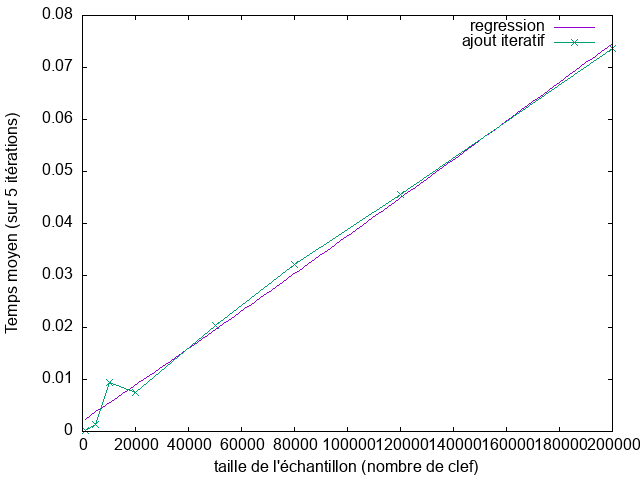
\includegraphics[width=5cm]{../Images/svg courbes pour rapport/regression_ajout_iteratif_arbre.png}
\caption{Tas sous forme d'arbre}
\label{fig2}
\end{figure}
  
  
  \end{column}
 \end{columns}  



\end{frame}

\begin{frame}{Construction}
Formule pour la régression : $(ax +b)$

\begin{columns}[t]
  \begin{column}{5cm}
  
\begin{figure}[hbtp]
\centering
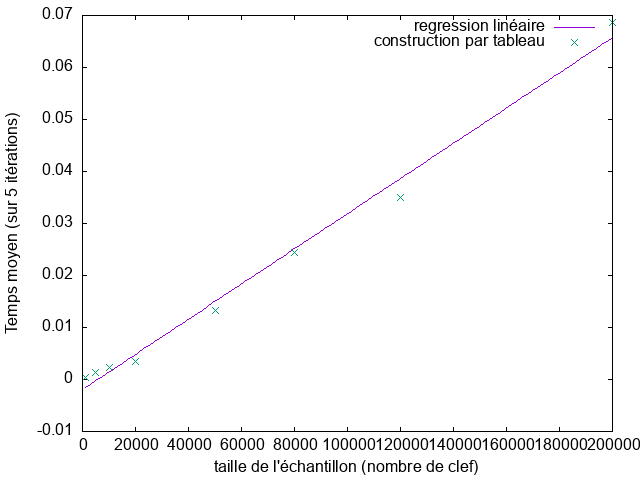
\includegraphics[width=5cm]{../Images/svg courbes pour rapport/cplxt_cons_tab_regression.png}
\caption{Tas sous forme de tableau}
\label{fig1}
\end{figure}


  \end{column}
  
  \begin{column}{5cm}
  
\begin{figure}[hbtp]
\centering
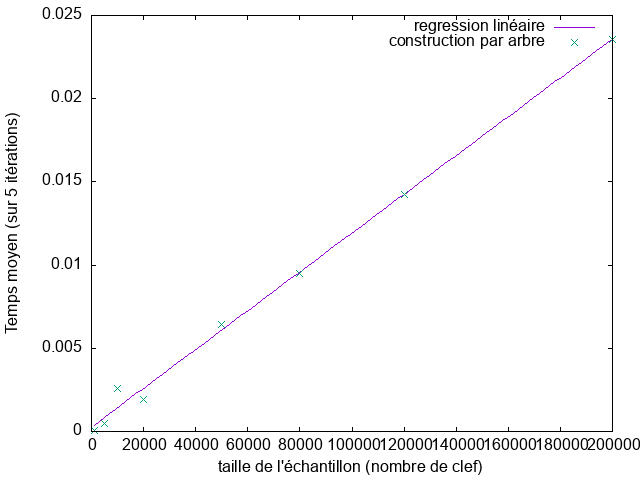
\includegraphics[width=5cm]{../Images/svg courbes pour rapport/cplxt_cons_arbre_regression.png}
\caption{Tas sous forme d'arbre}
\label{fig2}
\end{figure}
  
  
  \end{column}
 \end{columns}  



\end{frame}

\begin{frame}{Union}

\begin{columns}[t]
  \begin{column}{5cm}
  
\begin{figure}[hbtp]
\centering
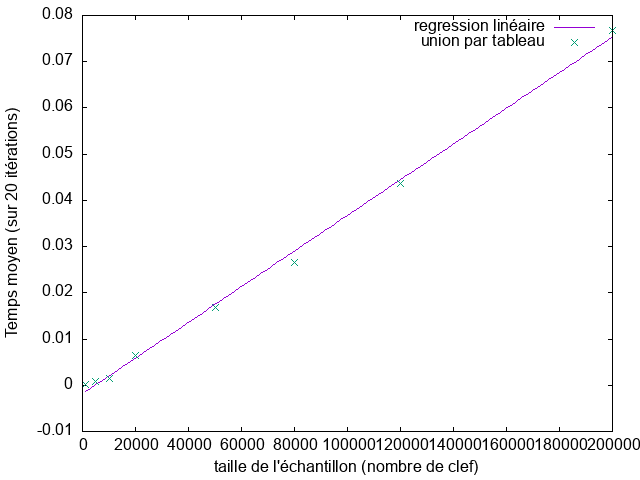
\includegraphics[width=5cm]{../Images/svg courbes pour rapport/cplxt_union_tab_regression.png}
\caption{Tas sous forme de tableau}
\label{fig1}
\end{figure}


  \end{column}
  
  \begin{column}{5cm}
  
\begin{figure}[hbtp]
\centering
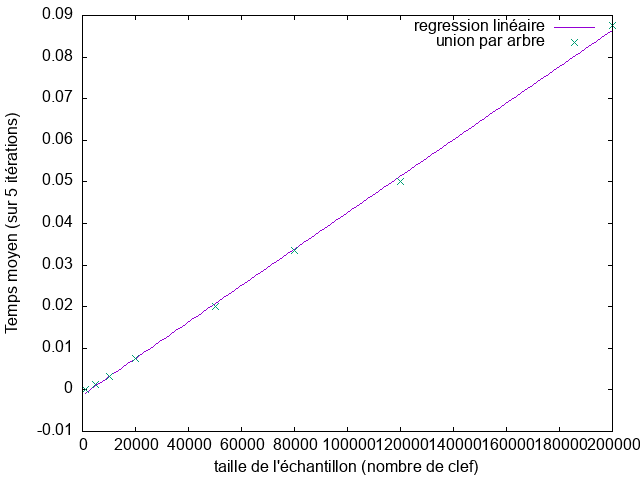
\includegraphics[width=5cm]{../Images/svg courbes pour rapport/cplxt_union_arbre_regression.png}
\caption{Tas sous forme d'arbre}
\label{fig2}
\end{figure}
  
  
  \end{column}
 \end{columns}  



\end{frame}

\section{File Binomiale}

\begin{frame}[fragile]{Implémentation}

\bigskip \begin{lstlisting}
(*Racine(degre,cle,fils)*)
type tournois_b = Racine of int * Int128.t * (tournois_b list)  | Empty 
(*File(indice,tournois) tournois le plus petit a gauche de la liste *) 
type file_b = File of int * (tournois_b list) | Empty 
\end{lstlisting} \bigskip

\end{frame}


\subsection{Complexités}


\begin{frame}{Construction et union}

\begin{columns}[t]
  \begin{column}{5cm}
  
\begin{figure}[hbtp]
\centering
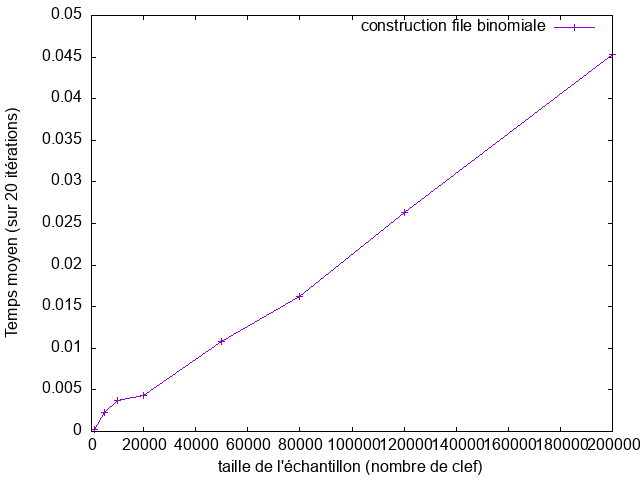
\includegraphics[width=5cm]{../Images/svg courbes pour rapport/cplxt_binomiale.png}
\caption{Complexité de la construction}
\label{fig1}
\end{figure}


  \end{column}
  
  \begin{column}{5cm}
  
\begin{figure}[hbtp]
\centering
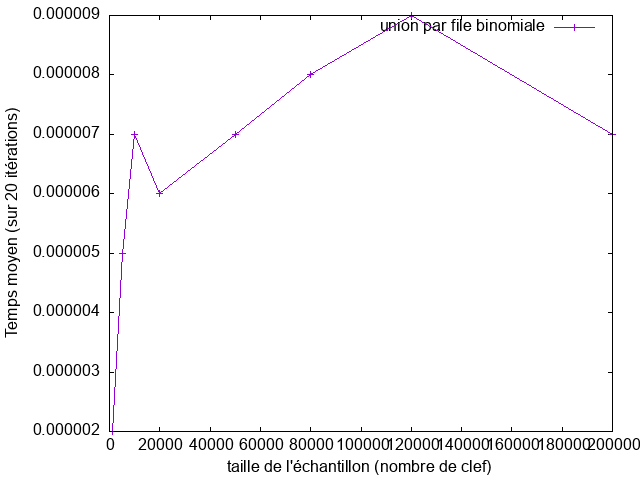
\includegraphics[width=5cm]{../Images/svg courbes pour rapport/cplxt_union_file.png}
\caption{Complexité de l'union}
\label{fig2}
\end{figure}
  
  
  \end{column}
 \end{columns}  



\end{frame}






\section{Hachage md5}


\begin{frame}[fragile]{Implémentation\cite{md5}}
\begin{lstlisting}
    val get_int32_le : string -> int -> int32
\end{lstlisting}  
\begin{lstlisting}
let finish (entre : int32) : int32 =
  let res = 0l in
  let res = Int32.logor res (Int32.shift_left (Int32.logand entre 0x000000FFl) 24) in 
  let res = Int32.logor res (Int32.shift_left (Int32.logand entre 0x0000FF00l) 8) in 
  let res = Int32.logor res (Int32.shift_right_logical (Int32.logand entre 0x00FF0000l) 8) in 
  let res = Int32.logor res (Int32.shift_right_logical (Int32.logand entre 0xFF000000l) 24) in 
  res
;;
\end{lstlisting} 

\end{frame}

\begin{frame}{Collisions}

\begin{align}
\mathbb{P} &= 1 - \prod_{i = 0}^{n -1} ( 1 - \frac{i}{m})\\
&= 1 - exp \prod_{i = 0}^{n -1} ln( 1 - \frac{i}{m})\\
&\approx 1 - e^{-\frac{n^2}{2m}}
\end{align}

\begin{itemize}
\item $m = 2^{128}$ (nombre de clés possibles codées sur 128 bits)
\item $n \approx 271000$ (nombre de mots de la langue anglaise)
\end{itemize}

$$\mathbb{P}\approx 1 - e^{-\frac{7,3441\times10^{10}}{2^{129}}} \approx 1,0791\times10^{-28}$$


\end{frame}

\section{Arbre de recherche}

\begin{frame}[fragile]{Choix et et implémentation}

\bigskip \begin{lstlisting}
type arbre234 = 
  | Empty
  | Feuille1 of Int128.t
  | Feuille2 of Int128.t * Int128.t
  | Noeud2 of Int128.t * arbre234 * arbre234 
  | Noeud3 of Int128.t * Int128.t * arbre234 * arbre234 * arbre234 
  | Noeud4 of Int128.t * Int128.t * Int128.t * arbre234 * arbre234 * arbre234 * arbre234 
\end{lstlisting} 

\bigskip \begin{lstlisting}
exception Eclatement of 
(Int128.t * arbre234 * arbre234) ;;
\end{lstlisting} \bigskip


\end{frame}

\section{Expérimentations et conclusions}


\begin{frame}[fragile]{Récupérer la liste de mots}

\begin{lstlisting}
let filtredroite (ligne : string ) : string = (*...*)

let filtregauche (ligne : string ) : string = (*...*)

let extraire_liste (nom : string) 
	(liste : Int128.t list)
	 (arbre : Arbre_234.arbre234) :
	  Int128.t list* Arbre_234.arbre234 = (*...*)

let extraire_liste_rep (path_rep : string) : Int128.t list = (*...*)
\end{lstlisting}


\end{frame}




\begin{frame}{Comparaison de nos structures}

\begin{columns}[t]
  \begin{column}{5cm}
  
\begin{figure}[hbtp]
\centering
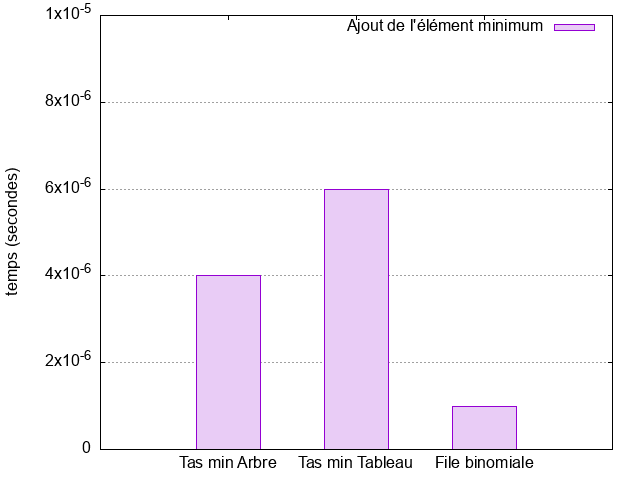
\includegraphics[width=5cm]{../Images/svg courbes pour rapport/temps_ajout_shakespeare.png} 
\caption{Ajout}
\label{fig1}
\end{figure}


  \end{column}
 
  \begin{column}{5cm}

\begin{figure}[hbtp]
\centering
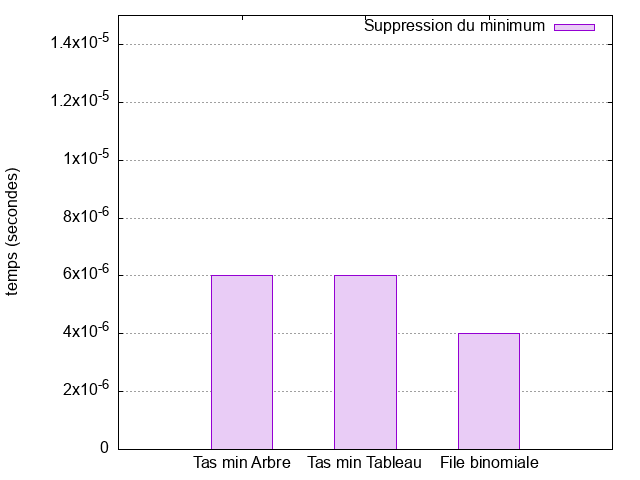
\includegraphics[width=5cm]{../Images/svg courbes pour rapport/temps_suppr_shakespeare.png} 
\caption{Suppression du minimum}
\label{fig1}
\end{figure}

  \end{column}
 \end{columns}  

\end{frame}



\begin{frame}{Comparaison de nos structures (suite)}

\begin{columns}[t]
  \begin{column}{5cm}
  
\begin{figure}[hbtp]
\centering
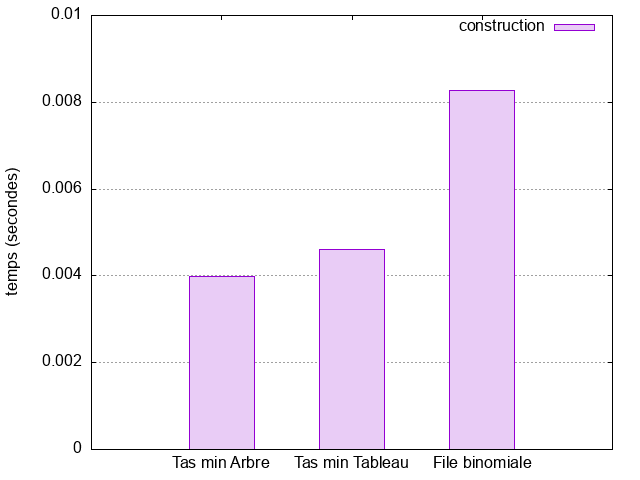
\includegraphics[width=5cm]{../Images/svg courbes pour rapport/temps_construction_shakespeare.png} 
\caption{Construction}
\label{fig1}
\end{figure}


  \end{column}
 
  \begin{column}{5cm}

\begin{figure}[hbtp]
\centering
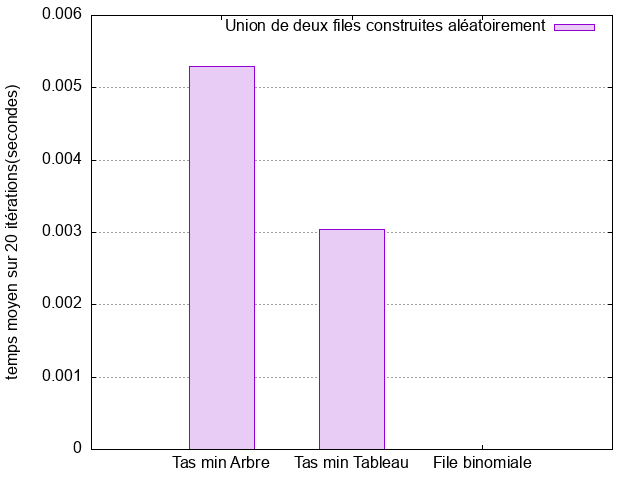
\includegraphics[width=5cm]{../Images/svg courbes pour rapport/temps_union_shakespeare.png} 
\caption{Union}
\label{fig1}
\end{figure}

  \end{column}
 \end{columns}  


\end{frame}

\begin{frame}
\bibliography{biblio.bib}
\bibliographystyle{plain}
\end{frame}


\end{document}